\documentclass[11pt,a4paper]{article}

\usepackage{xcolor}
\usepackage{graphicx}
\usepackage{hyperref}
\usepackage{amsmath}
\usepackage{cleveref}
\usepackage{footnote}
% \usepackage[bottom]{footmisc} % make footnotes go to the bottom
% \usepackage{natbib}
\usepackage{booktabs}
%
% File acl2020.tex
%
%% Based on the style files for ACL 2020, which were
%% Based on the style files for ACL 2018, NAACL 2018/19, which were
%% Based on the style files for ACL-2015, with some improvements
%%  taken from the NAACL-2016 style
%% Based on the style files for ACL-2014, which were, in turn,
%% based on ACL-2013, ACL-2012, ACL-2011, ACL-2010, ACL-IJCNLP-2009,
%% EACL-2009, IJCNLP-2008...
%% Based on the style files for EACL 2006 by 
%%e.agirre@ehu.es or Sergi.Balari@uab.es
%% and that of ACL 08 by Joakim Nivre and Noah Smith

\usepackage[hyperref]{acl2020}
\usepackage{times}
\usepackage{latexsym}
\renewcommand{\UrlFont}{\ttfamily\small}

% This is not strictly necessary, and may be commented out,
% but it will improve the layout of the manuscript,
% and will typically save some space.
\usepackage{microtype}

\aclfinalcopy % Uncomment this line for the final submission
%\def\aclpaperid{***} %  Enter the acl Paper ID here

%\setlength\titlebox{5cm}
% You can expand the titlebox if you need extra space
% to show all the authors. Please do not make the titlebox
% smaller than 5cm (the original size); we will check this
% in the camera-ready version and ask you to change it back.

\title{Leveraging Neural MT Output for Word Alignment}
\author{Vilém Zouhar \\ zouhar@ufal.mff.cuni.cz}
% \date{}

\begin{document}

\newcommand{\footnotehref}[2]{\footnote{\href{#1}{#2}}}
\newcommand{\rec}[1]{\textcolor{violet}{RECOMPUTE #1}}
\newcommand{\TODO}[1]{\textcolor{red}{TODO: #1}}
\newcommand{\DTODO}[1]{\textcolor{red}{Daria TODO: #1}}
\newcommand{\fastalign}{fast\_align}

\maketitle

\begin{abstract}
The most common tools for word alignment rely on a large amount of parallel sentences, which are then processed in usually one of the IBM Model algorithms. The training data is, however, the same as for machine translation (MT) systems, especially for neural MT (NMT), which itself is able to produce word alignments using the trained attention heads. This is convenient because word alignment is theoretically a viable byproduct of any attention-based NMT.

We summarize different approaches in which word alignment can be extracted from alignment scores and then explore ways in which scores can be extracted from NMT, focusing on inferring the word alignment scores based on output sentence and token probabilities. We compare this to extracting alignment scores from attention.

We conclude with aggregating all of the sources of alignment scores into a simple feed-forward network, which achieves the best results when combined alignment extractors are used.
\end{abstract}

\section{Introduction}

We first present (in a very introductory manner) the task of word-alignment and the used tools. In two parts of the evaluation, we first present and evaluate simple word alignment models individually (\Cref{sec:individual}) and then enhanced with new features and combined together using a neural network (\Cref{sec:aggregated}). In both cases, we explore the models' behaviour on Czech-English and German-English datasets.

All of the code is available\footnotehref{https://github.com/zouharvi/LeverageAlign}{github.com/zouharvi/LeverageAlign} open-source.

\subsection{Word Alignment}

Word alignment (also bitext alignment) is a task of matching two groups of words together that are each other's semantic translation. This is, of course, problematic for non-content words, which are specific for the given language, but generally one is able to construct a mapping as in the example in \Cref{fig:alignment_example}. Word alignment usually follows after sentence alignment.  Even though it is called word alignment, it usually operates also on tokens.
% \footnote{Drawn using \href{https://vilda.net/s/slowalign/}{vilda.net/s/slowalign}. More complex word alignment illustrations are available with \href{https://github.com/M4t1ss/SoftAlignments}{github.com/M4t1ss/SoftAlignments}}

\begin{figure*}[h!]
    \center
    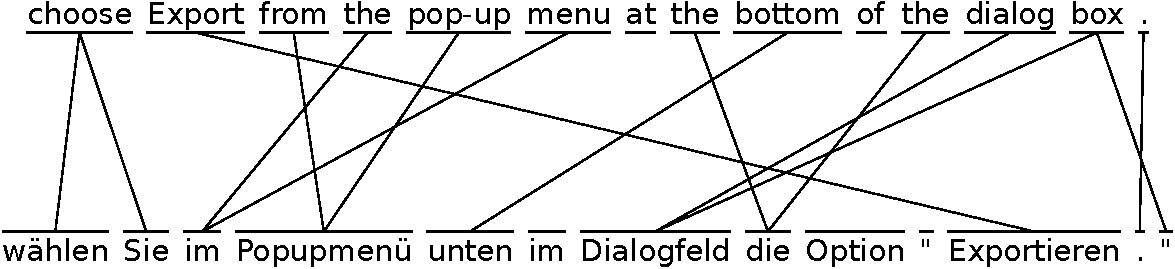
\includegraphics[width=0.75\textwidth]{img/alignment_example.pdf}
    \caption{
        Illustration of English-German word alignment. Source token \textit{choose} is aligned to two target tokens \textit{wählen} and \textit{Sie}, while the target token \textit{Option} is left unaligned. The target article \textit{die} is mistakenly aligned to two unrelated articles \textit{the}.
        \label{fig:alignment_example}
    }
\end{figure*}

Although word alignment found its use mainly in phrase-based machine translation (for generating phrase tables), it is still useful for many other tasks and applications: boosting MT performance \citep{alkhouli2016alignment}, exploring cross-linguistic phenomena \citep{schrader2006does}, computing quality estimation \citep{specia2013quest}, presenting quality estimation \citep{zouhar2020extending} or simply highlighting matching words and phrases in interactive MT (publicly available MT services).

Word alignment output can be formalized as a set containing tuples of source and target words. For output $A$ and gold alignment $G$, precision can be computes as: $ |A \cap G| / |A|$ and recall as $|A \cap G| / |G|$. F score is defined in a standard manner. These evaluation measures are very well described by \citet{mihalcea2003evaluation}.

\subsection{Relevant Work}

The work of \citet{li2019word} is closely related to this article, as it systematically examines the issue of word alignment from NMT and proposes two ways of extracting it: prediction difference and explicit model. They also show that without guided alignment in training, NMT systems perform worse than \fastalign{} baseline.

\subsection{Tools}

For the purposes of this experiment, we need two main tools: IBM model based word aligner and an MT system capable of providing output probabilities and optionally also attention-based word alignment.

\paragraph{\fastalign} \citep{dyer2013simple} is a word aligner based on IBM Alignment Model 2. It does not provide state of the art pre-neural performance but is easy to build with modern toolchains and has low resource requirements (both memory- and computational-wise).

\paragraph{MarianNMT} \citep{junczys2018marian} is a popular (both in academia and in deployment scenarios) actively developed and maintained system for machine translation. It already contains options for producing word alignment and output probabilities.

\subsection{Data}

For training purposes, we make use mostly of the manually annotated parallel corpora of word alignment Czech-English by \citet{marecek_csen_algn_corpus}. We also include German-English Big corpus by \citet{rozis_tilde}, which has not been word-aligned. From this corpus, 1M sentences were sampled randomly. The manually aligned German-English Small corpus by \citet{bicini_ende_algn_corpus} is included for testing. Overview of the corpus sizes is shown in \Cref{tab:corpus_used}.

\begin{table*}[h!]
    \center
    \begin{tabular}{lccccc}
        \toprule
        CS/DE-English & Type & Domain &\hspace{-0.1cm}CS/DE Tokens & EN Tokens & Sentences \\
        \cmidrule{1-6}
        Czech- & aligned & news, legal & 106k & 119k & 5k \\
        German- Small\hspace{-0.2cm} & aligned & legal & 1445 & 1478 & 100 \\
        German- Big & unaligned &tech, news, legal & 23M & 24M & 1M \\
        \bottomrule
    \end{tabular}
    \caption{Used word aligned corpora with their sizes, domains and origin. \label{tab:corpus_used}}
\end{table*}

\subsection{MT Models}

We make use of the MT models made available\footnotehref{https://github.com/browsermt/students}{github.com/browsermt/students} by the \citet{model_csen} and \citet{model_deen}. For both Czech-English and English-German, CPU-optimized student models are used. They are transformer based \citep{vaswani2017transformer} and were created by knowledge distillation, as proposed by \citet{germann-EtAl:2020:WMT}. With WM18 SacreBLEU \citep{sacrebleu}, the models achieve the following BLEU scores: Czech-English (32.6), English-Czech (27.9) and English-German (46.4).
\section{Individual Models} \label{sec:individual}

In this section, we describe and evaluate the individual word alignment models. All of the newly introduced models make use of the fact that NMT systems can be viewed as language models and can produce translation probabilities.

\subsection{Baseline Models} \label{subsec:baseline_models}

The first model is \fastalign{}. The second is attention-based soft word alignment extracted from MarianNMT (Attention), which was trained with guided alignment during the distillation. For the rest of this subsection, we will focus on models generating soft alignment scores (an unbounded real number corresponding to the quality of a possible alignment between two tokens) and not the alignments themselves.

\paragraph{One Token Translation ($M_1$).}

The simplest approach to get alignment scores is to compute decoder translation probability using the MT (function $m$) between every source and target token $s_i$ and $t_j$ of the source and target sentences $S$ and $T$. Single tokens are passed to the models as if they were a sentence pair. The scores are not normalized which is not an issue in this case, since the models working with these alignment scores (in \Cref{subsec:extractors}) compare output from sequences of the same length.
\begin{gather*}
\forall s_i\in S, t_j \in T: p(s_i, t_j) = m(\{s_i\}, \{t_j\})
\end{gather*}

The produced values are in a log space $(-\inf, 0]$. This approach requires $|S|\cdot |T|$ of one-token translation scorings (decoder probability of the target reference) for producing word alignments of a single sentence pair. On a CPU,\footnote{8 threads 2.3GHz Ryzen 7 3700u, no RAM to disk swapping} the models average to $2.7$s per one sentence pair alignment.

\paragraph{Source Token Dropout ($M_2$).}

A more refined approach was chosen by \citet{zintgraf2017visualizing} in which the alignment score is computed as the difference in target token probability when the source token is unknown. The exact approach is too computationally demanding (requires translation scorings with large amounts of replacement words), and therefore we use a much simpler, yet conceptually similar method by either omitting the token or replacing it with \texttt{<unk>}.\footnote{Even though subword-based MT models do not need \texttt{<unk>}, SentencePiece reserves the token \texttt{<unk>} for an unknown symbol.}
Assume $m_j(S, T)$ produces the log probability of the $j$-th target token. The sentence $S^{a/b}_i$ with an obscured token $s_i$ can be defined in two ways which leads to two versions of this model: $M_2^a$ and $M_2^b$. Output is then possibly unbounded $(-\inf,\inf)$.
\begin{gather*}
    \forall s_i \in S, t_j \in T: p(s_i, t_j) = m_j(S, T) - m_j(S^{a/b}_i, T)
\end{gather*}

\vspace{-0.8cm}

\begin{align*}
    & \text{Word deletion}\, (M_2^a): 
    & S^{a}_i = s_0, s_1, \ldots, s_{i-1}, s_{i+1}, \ldots, s_{|S|} \\
    & \text{Word substitution}\, (M_2^b):
    & S^{b}_i = s_0, s_1, \ldots, s_{i-1}, \texttt{<unk>}, s_{i+1}, \ldots, s_{|S|}
\end{align*}

This requires $|S|$ translation scorings of source and target lengths $|S|$ and $|T|$, which is comparable to $M_1$. The models average to $1.5$s per one sentence pair alignment.\footnote{ The running time is lower because in this case it is $|S|$ scorings of length $|T|$, while in $M_1$ it is $|S|\times|T|$ scorings of length $1$.}

\paragraph{Source and Target Dropout ($M_3$).}

A very similar method would be to also dropout the target token and examine how the sentence probability changes. Applying the two different ways of dropout leads to four versions of this approach. Note that in this case we compute the sentence probability (because the target word is hidden) and also do not subtract from the base sentence probability, but rather use the new sentence probability as it is. This probability should be highest if the corresponding tokens are both obscured. The probability is in log space $(-\inf, 0]$.
\vspace{0.2cm}
\begin{gather*}
    \forall s_i \in S, t_j \in T: p(s_i, t_j) = m(S^{a/b}_i , T^{a/b}_j)
\end{gather*}

\vspace{-0.8cm}

\begin{align*}
    T^a_j &= t_0, t_1, \ldots, t_{j-1}, t_{j+1}, \ldots, t_{|T|} \\
    T^b_j &= t_0, t_1, \ldots, t_{j-1}, \texttt{<unk>}, t_{j+1}, \ldots, t_{|T|}
\end{align*}

\vspace{-0.8cm}

\begin{align*}
    & \text{Word deletion, deletion ($M_3^{aa}$)} & S^a_i, T^a_j \\
    & \text{Word deletion, substitution ($M_3^{ab}$)} & S^a_i, T^b_j \\
    & \text{Word substitution, deletion ($M_3^{ba}$)} & S^b_i, T^a_j \\  
    & \text{Word substitution, substitution ($M_3^{bb}$)} & S^b_i, T^b_j
\end{align*}

This approach requires $|S|\cdot|T|$ translation scorings of source and target lengths of $|S^{a/b}|$ and $|T^{a/b}|$ for sentence $S$ translated to $T$ which is roughly $|T|$ times more than in $M_1$ and $M_2$. This makes it it the most computationally demanding approach. On average it takes $46.1$s to produce one sentence pair alignment on a CPU.

\subsection{Direct Alignment from Baseline Models} \label{subsec:extractors}

All of the models (except for \fastalign{}) are not producing the alignments themselves, but soft alignment scores $p$ for each pair of tokens $(s, t)$ in source $S$ $\times$ target $T$ sentence. The hard alignment itself can then, for example, be computed in the following ways. The parameter $\alpha$ can be estimated from the development set. The function $p$ is in general any soft alignment function (e.g. attention scores or the alignment scores from IBM model 1 EM algorithm).

\begin{enumerate}
    \item For every source token $s$ take the target tokens $t$ with the maximum score.
    \begin{gather*}
        A_1 = \bigcup_{s \in S} \{ (s, t): p(s,t) = max_r \{p(s,r) \} \}
    \end{gather*}
    
    \item For every source token $s$ take all target tokens $t$ with a high enough score (above threshold). This method is used to control the density of alignments in the work of \citet{liang2006alignment} and provides a parameter to tradeoff precision and recall.
    \begin{gather*}
        A_2^\alpha = \bigcup_{s \in S} \{(s, t): p(s,t) \ge \alpha \}
    \end{gather*}
    
    \item For every source token $s$ take any target token which has a score of at least $\alpha$ times the score of the best candidate. Special handling for negative cases in the form of a division is required to make the formula work for the whole $\mathbb{R}$. The motivation for this is $M_2$, which provides possibly unbounded alignment scores. Assume $\alpha \in (0, 1]$.
    \begin{gather*}
        A_3^\alpha = \bigcup_{s \in S} \{ (s, t): p(s,t) \ge min
        \big[ \max_r\ p(s,r) \cdot \alpha, \max_r\ p(s,r)\, /\, \alpha \big] \}
    \end{gather*}
    $A_1$ can then be expressed as $A_3^1$. Lower $alpha$ values lead to lower precision and higher recall because the algorithm includes more, less probable, alignments. A variation on this approach would be to subtract $\alpha$ instead of multiplying it. The reason for choosing multiplication is that it dynamically adapts to a wider range of intervals and bounds the parameters between $0$ and $1$. This is not the case for substraction and because of this, it would be harder to choose the right parameter. 
    
    \smallskip
    \item Similar approach is for $A_3$, but with the focus on the target side. For every target token $t$ take any source token which has a score of at least $\alpha$ times the score of the best candidate.
    \begin{gather*}
        A_4^\alpha = \bigcup_{t \in T} \{ (s, t): p(s,t) \ge min
        \big[ \max_r\ p(r,t) \cdot \alpha, \max_r\ p(r,t) / \alpha \big] \}
    \end{gather*}
    Similar reversal for $A_2$ would not make sense, because it already takes all alignment above a threshold without any consideration for the direction.
    
    \item Similarly to $M_3$ and $M_4$ it is possible to create an extractor in which instead of having a single dropout on the target side, there are a multiple of them. This way, the score would not be between the source token and the target token, but between the source token and a subset of all target tokens. Formally, this would replace the (complete) weighted graph structure with a (complete) hypergraph. Instead of just having a weight for \textit{Choose--Wählen}, there would also be a weight for \textit{\{Choose\}--\{Wählen, Sie\}}, \textit{\{Choose\}-\{Wählen, im, Popupmenü\}} etc. 
    This would, however, lead to exponential complexity in terms of target sentence length. The number of words participating in an edge would then have to be limited to the number of alignments to a single token that we can empirically expect of the given language pair. \Cref{fig:alignment_example} suggests that for English-German this could be 3.
    Upon computing the scores for all the edges in this hypergraph, a follow-up task would be to find the maximum-weight matching.
\end{enumerate}

\vspace{-0.4cm}
\paragraph{Coverage.}

The suggested greedy way of computing alignments from alignment scores is far from perfect.
In the scenario depicted in \Cref{fig:alignment_coverage}, all but the last source token (German) have been aligned with the target, each with different alignment scores. Although the model may lack any lexical knowledge of the word \textit{Übersetzung}, it should consider the prior of a word being aligned to at least one target token.

\begin{figure}[h!]
    \center
    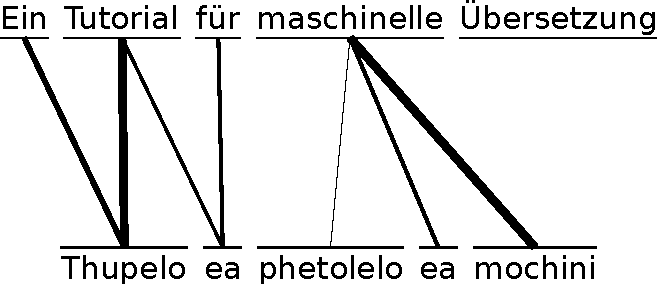
\includegraphics[width=0.5\textwidth]{alignment_coverage.pdf}
    \caption{
        Partial alignment from German (top) to Sesotho (bottom). The model has no lexical knowledge about the alignment of >>Übersetzung<<, though >>phetolelo<< is a good candidate because no other word aligned to it. Line strength corresponds to the soft alignments produced by the model.
        \label{fig:alignment_coverage}
    }
\end{figure}

In this specific case, $A_3^{0.9}$ would probably include all alignments to the word \textit{Übersetzung}, since there is no single strong candidate (assume that lines not visible depict soft alignments close to $0$). Similarly, $A_4^{0.9}$ would also include most alignments of the word \textit{Übersetzung}, including the word \textit{phetolelo}, since the alignment score with \textit{maschinelle} is weak and also close to $0$. Intersecting these two extractors $A_3^{0.9} \cap A_4^{0.9}$ would yield the correct alignment \textit{Übersetzung--phetolelo}. Other tokens would not be aligned to either of these two words because they have strong alignment scores with different tokens.

This prior may not always be desirable. For this, intersecting with $A_2^\alpha$ provides a limiting threshold. In an application where the target token is erroneous, this prevents the alignment model from aligning the two corresponding tokens.
Inducing alignment based on graph properties is examined by \citet{symmetric}, though without the presence of NMT.
\section{Ensembling of Individual Models} \label{sec:aggregated}

In the previous section, we saw that multiple methods with different properties achieved good results, but were sensitive to the method used to induce hard alignment. This section combines them together in a small feed-forward neural network, which can be trained on a small amount of data.

\subsection{Model}

The ensemble neural network itself is a regressor: $\mathbf{F} \rightarrow (0, 1)$, where $\mathbf{F}$ is the set of feature vectors for every pair of source and target tokens.\footnote{A completely different approach would be to simply use (pretrained) word embeddings as an input to the network. This is, however, not possible due to the low amount of gold alignment data.} By applying sigmoid to the output and establishing a threshold value for the positive class, the network would become a classifier. This behaviour can, however, be simulated using $A_2^\alpha$. We work with the threshold explicitly and use the network for computing alignment score and not for the alignment itself.
For the hard alignment, we use $A_2^{0.001} \cap A_3^{1} \cap A_4^{1}$, which we found to work the best with this ensemble on the training data.

\paragraph{Additional Features.} Apart from $M_1$, $M_2^b$, $M_3^{aa}$, $M_3^{bb}$ and Attention with averaging aggregation (Individual), we also include the output of \fastalign{} as one of the features. Moreover, four other manually crafted features (Manual) are added. The motivation for the first two manual features is that the position and token length help in determining the alignment in some cases. The last two are specifically targeted at named entities, which have sparse occurrences in the data, and also at non-word tokens, such as full stops, delimiters and quotation marks. 
We list Pearson's correlation coefficient with true alignments on Czech$\leftrightarrow$English data (the two directions averaged).

\smallskip
\begin{itemize}
    \item Difference in sentence positions:\\
    $\rho = \text{-}\ 0.18$, \qquad $abs(\,i/|S|-j/|T|\,)$ 
    \item Difference in token lengths:\\
    $\rho = \text{-}\ 0.11$, \qquad $abs(\,|s_i|-|t_j|\,)$ 
    \item Difference in subword unit counts:\\
    $\rho = \text{-}\ 0.03$, \qquad $abs(\,|\text{subw}(s_i)|-|\text{subw}(t_j)|\,)$ 
    \item Normalized token case-insensitive Levenshtein distance:\\
    $\rho = \text{-}\ 0.30$, \qquad $lev(s_i, t_j)/max(|s_i|, |t_j|)$
    \item Number of subword units which are present in both tokens:\footnote{Normalized version of this feature had slightly lower correlation coefficient: $0.30$.}\\
    $\rho = \,\,\,0.32$, \qquad $|\,\text{subw}(s_i) \cap \text{subw}(t_j)\,|$
    \item Token string case-insensitive equality (equal to zero Levenshtein distance):\\
    $\rho = \,\,\,0.28$, \qquad $I_{s_i \simeq t_j}$
\end{itemize}

\paragraph{Architecture.} For every model, the epoch with the lowest AER on the validation dataset is used for the test dataset. This extractor was found to work best across all ensemble models. The training was done with cross-entropy loss. The model was composed of series of hidden linear layers, each with biases and Tanh as the activation function with dropouts around the innermost layer:
\begin{gather*}
    L_{|\text{Input}|}^\text{Tanh}\circ L_{32}^\text{Tanh} \circ D_{0.2} \circ L_{16}^\text{Tanh} \circ D_{0.2} \circ L_{16}^\text{Tanh} \circ L_{8}^\text{Tanh} \circ L_1^\text{Softmax}
\end{gather*}

\subsection{Data}

The Czech$\leftrightarrow$English dataset contains 1.5M source-target pairs, out of which $2.64\%$ is of a positive class (aligned). For German$\leftrightarrow$English Small these quantities are 22k and $5.61\%$ respectively. This could be an issue for a simple classifier network and would need e.g. oversampling of the positive or undersampling of the negative class.

For Czech$\leftrightarrow$English, we used $10\%$ and $10\%$ (250 sentences each) for validation and test data and the rest for training. Samples were split on sentence boundaries. The English$\rightarrow$German was used solely for testing, due to its small size.

\subsection{Evaluation}

The averaged results of each ensemble on Czech$\leftrightarrow$English are in \Cref{tab:ensemble_performance}. We also show the results of $M_1$, but without $A_2$. Due to the range of $M_1$'s values, it is difficult to establish a cut-off threshold. Attention uses $A_3^1$, since intersection with other extractors did not improve the performance, as described in \Cref{sec:evaluation}.
The results demonstrate that adding any feature improves the overall ensemble. All features combined together improve on the best individual model by $-0.11$\, AER.\footnote{Performed by Student's t-test on 10 runs with $p<0.001$.}

\newcommand{\staroff}{\hspace{0.02cm}$\star$\hspace*{-0.28cm}}
\begin{table*}[h!]
    \center
    \begin{tabular}{lccc}
        \toprule
        Model\,/\,Features & Precision & Recall & AER \\
        \midrule
        $M_1$ ($A_3^{1} \cap A_4^{1}$) & $0.75$ & $0.78$ & $0.25$ \staroff \\
        Attention (max, $A_3^1$) & $0.64$ & $0.81$ & $0.29$ \\
        \fastalign{} Small & $0.54$ & $0.66$ & $0.41$ \\
        \fastalign{} Big & $0.63$ & $0.64$ & $0.38$ \\
        \midrule
        Manual features & $0.55$ & $0.46$ & $0.50$ \\
        Individual ($M_1$, $M_2^b$, $M_3^{aa}$, $M_3^{bb}$, attention) &  $0.84$ & $0.73$ & $0.23$ \\
        Manual + Indiv. & $0.85$ & $0.79$ & $0.19$ \\
        Manual + Indiv. + \fastalign{} & $0.86$ & $0.79$ & $0.18$ \\
        Manual + Indiv. + \fastalign{} + Attention & $0.85$ & $0.84$ & $0.16$ \\
        Manual + Indiv. + \fastalign{} + Attention + M1 rev. \hspace*{-0.4cm} & $0.86$ & $0.86$ & $0.14$ \staroff \\
        \bottomrule
    \end{tabular}
    \caption{Average Precision, Recall and AER of $M_1$ (best individual) and different ensemble models (using $A_2^{0.001} \cap A_3^{1} \cap A_4^{1}$) on Czech$\leftrightarrow$English data (averaged) \label{tab:ensemble_performance}}
\end{table*}

\vspace{-0.2cm}
\paragraph{Transfer.} The best models on Czech$\leftrightarrow$English (one for each direction) were then used on the English$\rightarrow$German dataset, resulting on average in AER = $0.18$. This is higher than for Czech but still significantly lower (by a margin of $-0.08$)\footnote{Performed by Student's t-test with $p<0.001$.} than for the best individual model, Attention (max). This suggests that the features generalize well and models can be trained even on other language data. Furthermore, since the alignment datasets come from different origins, there may be systematic biases, which lower the performance of the transfer.
\section{Summary}

In this paper, we explored and compared different methods of inducing word alignment from trained neural machine translation models.

Despite its simplicity, estimating scores with single word translations (combined with reverse translations) appears to be the fastest and most robust solution, even in comparison to word-alignment from attention heads.

Ensembling individual model scores with a simple feed-forward network improve the final performance to $F_1 = 0.86$ on Czech$\leftrightarrow$English data.

\subsubsection*{Future work}

In \Cref{subsec:baseline_models} we presented but did not explore an idea of target dropout with multiple target tokens missing in order to better model the fact that words rarely map 1:1.

Throughout the experiment, we used neural machine translation for providing alignment scores but then used a primitive extractor algorithm for obtaining hard alignment. More sophisticated extractor approaches, which take into consideration the alignment score origin (neural MT), could vastly improve the performance.

Furthermore, we did not examine the possible effects of fine-tuning the translation model on the available data.

\section*{Acknowledgements}

This article has used extensively resources made available by the H2020-ICT-2018-2-825303 (Bergamot) grant.

\bibliography{citations}
\bibliographystyle{acl_natbib}

\end{document}
